\begin{savequote}[45mm]
Gauge symmetry principles are regularly invoked in the context of justification, as deep physical principles, fundamental starting points in thinking about why physical theories are the way they are, so to speak.  
\qauthor{“On continuous symmetries and the foundations of modern physics” by Christopher A. Martin}
\end{savequote}
\chapter{Multiple Particles}
\label{ch:multiple_particles}
\section{Identical Particles: Two Particle Systems}
\subsection{Introduction}
Before we venture into multiple particle systems, let us investigate two particle systems, of which both the particles are identical to each other.\\
For two particle systems, the state is a function of coordinates of particle one $(\textbf{r}_1)$ and of particle two $(\textbf{r}_2)$ and the time,
\begin{equation}
    \Psi(\textbf{r}_1,\textbf{r}_2,t)
\end{equation}
Its time evolution is determined by the Schrodinger equation,
\begin{equation}
    i\hbar\frac{\partial \Psi}{\partial t}=\hat{H}\Psi
\end{equation}
where $H$ is the Hamiltonian for the whole system,
\begin{equation}
    \hat{H}=-\frac{\hbar^2}{2m_1}\nabla^2_1-\frac{\hbar^2}{2m_2}\nabla^2_2+V(\textbf{r}_1,\textbf{r}_2,t)
\end{equation}
The normalisation is done as always,
\begin{equation}
    \int\vert \Psi(\textbf{r}_1,\textbf{r}_2,t)\vert^2d^3\textbf{r}_1d^3\textbf{r}_2=1
\end{equation}
For time independent potentials, we obtain a complete set of solutions by separation of variables,
\begin{equation}
    \Psi(\textbf{r}_1,\textbf{r}_2,t)=\psi(\textbf{r}_1,\textbf{r}_2)e^{-iEt/\hbar}
\end{equation}
Where the spatial wavefunction $\psi$ satisfies the time-independent Schrodinger equation,
\begin{equation}
    -\frac{\hbar^2}{2m_1}\nabla^2_1\psi-\frac{\hbar^2}{2m_2}\nabla^2_2\psi+V\psi=E\psi
\end{equation}
Solving this equation is tedious, but two special cases can be considered, that can be reduced to one-particle problems.
\subsection{Non-interacting particles}
Suppose the particles do not interact with one another, but each is subject to some external force. In that case the total potential energy is the sum of the two,
\begin{equation}
    V(\textbf{r}_1\textbf{r}_2=V_1(\textbf{r}_1)+V_2(\textbf{r}_2)
\end{equation}
And so the Schrodinger equation for this potential can be solved by separation of variables,
\begin{equation}
    \psi_\textbf{r}_1,\textbf{r}_2)=\psi_a(\textbf{r}_1)\psi_b(\textbf{r}_2)
\end{equation}
Now, plugging this into the Schrodinger equation, dividing by $\psi_\textbf{r}_1,\textbf{r}_2$ and collecting terms, each satisfy the one-particle Schrodinger equation,
\begin{gather}
    -\frac{\hbar^2}{2m_1}\nabla^2_1\psi_a(\textbf{r}_1)+V_1(\textbf{r}_1)\psi_a(\textbf{r}_1)=E_a\psi_a(r_1)\\
     -\frac{\hbar^2}{2m_2}\nabla^2_1\psi_b(\textbf{r}_2)+V_2(\textbf{r}_2)\psi_b(\textbf{r}_2)=E_b\psi_b(r_2)
\end{gather}
and $E=E_a+E_b$. In this case, the two particle wavefunction is a simple product of one-particle wavefunctions,
\begin{gather}
    \Psi(\textbf{r}_1,\textbf{r}_2,t)=\psi_a(\textbf{r}_1)\psi_b(\textbf{r}_2)e^{i(E_a+E_b)t/\hbar}=\left(\psi_a(\textbf{r}_1e^{-iE_at/\hbar}\right)\left(\psi_a(\textbf{r}_1e^{-iE_at/\hbar}\right)\left(\psi_b(\textbf{r}_2e^{-iE_bt/\hbar}\right)
\end{gather}
Therefore
\begin{equation}
    \Psi(\textbf{r}_1,\textbf{r}_2,t)=\Psi_a(\textbf{r}_1,t)\Psi_b(\textbf{r}_2,t)
\end{equation}
And any linear combination of such solutions will still satisfy the Schrodinger equation, for example,
\begin{equation}
    \Psi_b(\textbf{r}_1\textbf{r}_2,t)=\frac{3}{5}\Psi_a(\textbf{r}_1,t)\psi_b(\textbf{r}_2,t)+\frac{4}{5}\Psi_c(\textbf{r}_1,t)\Psi_d(\textbf{r}_2,t)
\end{equation}
The state of particle 1 depends on the state of particle 2, and vice versa. We can say that the two particles are entangled. An entangled state is one that cannot be written as a product of single-particle states.
\subsection{Central Potentials}
Suppose the particles interact only with one another, via a potential that depends on their separation,
\begin{equation}
    V(\textbf{r}_1,\textbf{r}_2)\longrightarrow V(|\textbf{r}_2-\textbf{r}_2)
\end{equation}
The hydrogen atom would be an example, if you include the motion of the proton. In this case the two-body problem reduces to an equivalent one-body problem, just as it does in classical mechanics.\\
In general, though, the two particles will be subject both to external forces and to mutual interactions, and this makes the analysis more complicated.

\section{Bosons and Fermions}
Supposing that we have two non-interacting particles, the first particle in state $\psi_a()\textbf{r}$ and the second particle in state $\psi_b\textbf{r}$, then,
\begin{equation}
    \psi(\textbf{r}_1,\textbf{r}_2)=\psi_a()\textbf{r}\psi_b\textbf{r}
\end{equation}
These particles can be said to be indistinguishable in principle. This is not possible in classical mechanics, but quantum mechanics allows for this to be true.\\
Now, we can construct a wavefunction that is noncommittal as to which particle is in which state,
\begin{equation}
    \psi\pm (\textbf{r}_1\textbf{r}_2)=A[\psi_a(\textbf{r}_1\psi_b\textbf{r}_2\pm A[\psi_b(\textbf{r}_1\psi_a\textbf{r}_2]
\end{equation}
This theory admits two kinds of identical particles: the bosons and fermions. Boson states are symmetric under interchange, $\psi_+(\textbf{r}_2,\textbf{r}_1)=\psi_+(\textbf{r}_1/\textbf{r}_2)$, and the fermion states are anti-symmetric under interchange, $\psi_-(\textbf{r}_2,\textbf{r}_1)=-\psi_-(\textbf{r}_1/\textbf{r}_2)$
It follows that no two identical fermions can occupy the same state, if $\psi_a=\psi_b$, then,
\begin{equation}
    \psi_-(\textbf{r}_1\textbf{r}_2)=A[\psi_a(\textbf{r}_1)\psi_a(\textbf{r}_2)-\psi_a(\textbf{r}_1)\psi_a(\textbf{r}_2)]=0
\end{equation}
and we end up with a null wavefunction. This is the Pauli exclusion principle, and it applies not only to electrons, but to all fermions.
\section{Occupation Number representation}
The occupation number representation uses a different notation to describe a quantum system. We change the way we label states, and also replace the wavefunction with a version of creation and annihilation operators. This method requires the fundamental laws of indistinguishable particles that we looked at in the previous section,
\begin{itemize}
    \item There are only two types of particles- Bosons and fermions
    \item Exchanging two bosons gets you the same state
    \item Exchanging the two fermions gets you the minus of the initial state.
\end{itemize}
\subsection{Example: Particle in a box}
The momentum operator for motion along the x-direction can be written as,
\begin{equation}
    \hat{p}=-\frac{\partial}{\partial x}
\end{equation}
Now, we can deduce that the possible momentum states that the particles in the box can take are,
\begin{equation}
    p_m=\frac{2\pi m}{L}
\end{equation}
The possible momentum states are labelled $p_1.p_2,p_3$ and so on, and the energy of the particle in state $p_m$ is $E_{p_m}$.\\
We can make a simple many particle system by introducing many non interacting bosons in the box. To see the impact of these particles on the total momentum and energy of the system, we apply the momentum operator to the two particle state,
\begin{equation}
    \hat{p}|p_1p_2\rangle=(p_1+p_2)|p_1p_2\rangle
\end{equation}
And applying the Hamiltonian operator,
\begin{equation}
    \hat{H}|p_1p_2\rangle=(E_{p_1}+E{p_2})|p_1p_2\rangle
\end{equation}
The particles do not interact, hence having two particles in a particular energy state costs an energy $2E_{p_3}$, which is double the single particle energy.
\subsection{Changing the notation}
In quantum mechanics, we use the notation,
\begin{equation*}
    |ABC\rangle=|p_1p_2p_3\rangle
\end{equation*}
Which reads that particle A has momentum $p_1$ particle B has momentum $p_2$ and so on. Now using our axioms of indistinguishable particles, it negates the use of separate labelling of each particles. We also know that momentum can only have certain allowed values ($2\pi m/L$). We can define a state of N particles by listing how many are in each of the momentum states. Let us take an example,\\
\begin{figure}[H]
    \centering
    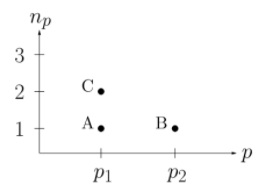
\includegraphics[scale=1]{Figures/occupation.png}
    \caption{A three particle system}
    \label{fig:my_label}
\end{figure}

In this example, we can write the states as $|2100\rangle$. This method is called the occupation number representation.\\
Now looking at the occupation number representation with the Hamiltonian,
\begin{equation}
    \hat{H}|n_1n_2n_3..\rangle=\left[\sum_m n_{p_m}E_{p_m}\right]|n_1n_2n_3...\rangle
\end{equation}
We simply multiply the number of particles in each state by the energy of that state and sum over all of the states.
\subsection{Replacing state vectors with operators}
Next, we are going to remove the state vector representations altogether using the same notation. We use operators to describe the physics rather than state vectors, and we retain only one special state, the vacuum state $|0\rangle$. Taking the harmonic oscillator for example, we can build up a general state of several harmonic oscillators by acting on the vacuum state $|0\rangle$,
\begin{equation}
    |n_1n_2...\rangle=\prod_{k}\frac{1}{(n_k!)}{^1/2}(\hat{a}^\dagger_k)^{n_k}|0\rangle
\end{equation}
Next, we need to verify if these creation and annihilation operators respect the exchange symmetry for identical particles.

\subsection{Indistinguishability and Symmetry}
Putting one particle in state $p_1$ and then another particle in $p_2$, or do the same thing in the reverse order, you should obtain the final state as $|11\rangle$. This means that,
\begin{equation}
    \hat{a}^\dagger_{p_1}\hat{a}^\dagger_{p_2}=\lambda\hat{a}^\dagger_{p_2}\hat{a}^\dagger_{p_1}
\end{equation}
We assume two cases, where $\lambda=\pm 1$, and they correspond to wavefunctions which are either symmetric or antisymmetric under particle exchange.\\
For bosons, $\lambda=1$
\begin{equation}
    \hat{a}^\dagger_{p_1}\hat{a}^\dagger_{p_2}=\hat{a}^\dagger_{p_2}\hat{a}^\dagger_{p_1}
\end{equation}
Rearranging and adding general labels,
\begin{equation}
    [\hat{a}^\dagger_{i}\hat{a}^\dagger_{j}]=[\hat{a}^\dagger_{i}\hat{a}^\dagger_{j}]-[\hat{a}^\dagger_{j}\hat{a}^\dagger_{i}]=0
\end{equation}
which means that the creation operators for different particle states commute. We also have the $[\hat{a}_i,\hat{a}_j]=0$, then,
\begin{equation}
    [\hat{a}_i,\hat{a}^\dagger_j]=\delta_{ij}
\end{equation}
This follows our harmonic oscillator commutation relations, and hence we can build up a state of many particles in momentum states using the formula,
\begin{equation}
     |n_1n_2...\rangle=\prod_{k}\frac{1}{(n_{p_m}!)^}{1/2}(\hat{a}^\dagger_{p_m})^{n{p_m}}|0\rangle
\end{equation}
The commutation of different operators implies that,
\begin{equation}
    \hat{a}^\dagger_{p_1}\hat{a}^\dagger_{p_2}|0\rangle=\hat{a}^\dagger_{p_2}\hat{a}^\dagger_{p_1}|0\rangle=|1_{p_1}1_{p_2}\rangle
\end{equation}
which means that it does not matter which order you put particles in the states, you get the exact same in all cases.\\
Generalising,
\begin{gather}
    \hat{a}^\dagger_i|n_1...n_i...\rangle=\sqrt{n_i+1}|n_1...n_i+1...\rangle\\
    \hat{a}_i|n_1...n_i...\rangle=\sqrt{n_i}|n_1...n_i-1...\rangle
\end{gather}
Now for fermions, we consider $\lambda=-1$, and so,
\begin{equation}
    \{\hat{c}^\dagger_i\hat{c}^\dagger_j\}\equiv \hat{c}^\dagger_i\hat{c}^\dagger_j+\hat{c}^\dagger_j\hat{c}^\dagger_i=0
\end{equation}
We can see that the fermion operators anti-commute, and when we set $i=j$, we find,
\begin{equation}
    \hat{c}^\dagger_i\hat{c}^\dagger_i+\hat{c}^\dagger_i\hat{c}^\dagger_i=0
\end{equation}
Which means that $\hat{c}^\dagger_i\hat{c}^\dagger_i=0$. This means that when we try to put two fermions in the same state, it annihilates it completely. This is the Pauli exclusion principle we saw previously, just with a change in notation. We also get,
\begin{equation}
    \{\hat{c}_i,\hat{c}_j\}=\delta_{ij}
\end{equation}
which means that we can use the harmonic oscillator analogy here as well, but note that order of placing the particle states matters in the case of fermions, because $\hat{c}^\dagger_i\hat{c}^\dagger_j|0\rangle=-\hat{c}^\dagger_j\hat{c}^\dagger_i|0\rangle$
\subsection{The continuum limit}
If we increase the size of the box, the momentum states become more closely spaced until the momentum a continuous variable. The Kronecker $\delta_{ij}$ functions become Dirac $\delta^{(3)}(\textbf{p})$ functions and the sums become integrals,
\begin{equation}
    \hat{a}_{\textbf{p}},\hat{a}^\dagger_{\textbf{q}}=\delta^{(3)}(\textbf{p}-\textbf{q})
\end{equation}
And for energies,
\begin{equation}
    \hat{H}=\int d^3pE_{\textbf{p}}\hat{a}^\dagger_{\textbf{p}}\hat{a}_{\textbf{p}}
\end{equation}
\section{Second Quantization}
\subsection{Field Operators}
Field operators create and annihilate particles in particular momentum states localised at particular spatial locations. Using Fourier sums, we can construct the field operator $\hat{\psi}^\dagger(x)$,
\begin{equation}
    \hat{\psi}^\dagger(x)=\frac{1}{\sqrt{\mathcal{V}}}\sum_{\textbf{p}}\hat{a}^\dagger_{\textbf{p}}e^{-i\textbf{p}\cdot\textbf{x}}
\end{equation}
creates a particle at position $x$, while $\hat{a}^\dagger_{\textbf{p}}$ creates a particle in a state with three-momentum $\textbf{p}$. Similarly the operator $\psi(\textbf{x})$ is defined by,
\begin{equation}
    \hat{\psi}(\textbf{x})=\frac{1}{\sqrt{\mathcal{V}}}\sum_{\textbf{p}}\hat{a}_{\textbf{p}}e^{i\textbf{p}\cdot\textbf{x}}
\end{equation}
annihilates a particle at position $x$, while $\hat{a}_{\textbf{p}}$ annihilates a particle in a state with three momentum $\textbf{p}$.
\subsection{Second quantization of single-particle operators}
We second quantize the n-particle operators by inserting the identities $1=\sum_\alpha=|\alpha\rangle\langle\alpha|$ and $1=\sum_\beta|\beta\rangle\langle\beta|$ into the right hand side of the identity $\hat{\mathcal{A}}=\hat{\mathcal{A}}$,
\begin{equation}
    \hat{\mathcal{A}}=\sum_{\alpha\beta}|\alpha\rangle\langle\alpha|\hat{\mathcal{A}}|\beta\rangle\langle\beta|=\sum_{\alpha\beta}\mathcal{A}_{\alpha\beta}|\alpha\rangle\langle\beta|
\end{equation}
where the matrix element $\mathcal{A}_{\alpha\beta}=\langle\alpha|\hat{\mathcal{A}}|\beta\rangle$.\\
The space that can accommodate multiple particle states is called Fock space, and it is simply defined by,
\begin{equation}
    \mathcal{F}=\bigoplus_{N=0}\mathcal{H}_N=\mathcal{H}_0\oplus \mathcal{H}_1\oplus...
\end{equation}
where $\mathcal{F}$ is the Fock space and the $\mathcal{H}_1$ and $\mathcal{H}_2$, and so on are the single particle Hilbert spaces.\\
The second-quantized version of operator $\hat{\mathcal{A}}$ is simply put as,
\begin{equation}
    \hat{A}=\sum_{\alpha\beta}\mathcal{A}_{\alpha\beta}\hat{a}^\dagger_\alpha\hat{a}_\beta
\end{equation}
What operator $\hat{A}$ essentially does is, it removes a single particle in state $|\beta\rangle$ by using the annihilation operator $\hat{a}_\beta$, multiplies it by the matrix element $\mathcal{A}_{\alpha\beta}$, and then uses $\hat{a}^\dagger_\alpha$ to place the particle into a final state $|\alpha\rangle$.
\subsection{Second quantization of two-particle operators}
The second quantized two particle operator is given by,
\begin{equation}
    \hat{A}=\sum_{\alpha\beta\gamma\delta}\mathcal{A}_{\alpha\beta\gamma\delta}\hat{a}^\dagger_\alpha\hat{a}^\dagger_\beta\hat{a}_\gamma\hat{a}_\delta
\end{equation}
This expression essentially is the sum over all the processes involving the annihilation of two particles in particular states, multiplication by the matrix element, and creation of the two particles in two new states.\\
The two particle operator can also be written in terms of spatial coordinates and field operators as,
\begin{equation}
    \hat{V}=\frac{1}{2}\int d^3xd^3y\hat{\psi}^\dagger(\textbf{x})\hat{\psi}^\dagger(\textbf{y})V(\textbf{x},\textbf{y})\hat{\psi}(\textbf{y})\hat{\psi}(\textbf{x})
\end{equation}
The factor $\frac{1}{2}$ ensures that we do not double count the interactions. We specifically order the operators by placing the creation operators to the left and the annihilation operators to the right, which is known as normal ordering. This makes sure that the operator $\hat{V}$ has zero vacuum expectation value,
\begin{equation}
    \langle 0|\hat{V}|0\rangle=0
\end{equation}
We also order the coordinates, because fermions anticommute, and mixing up the order of the coordinates might result in the wrong operator, but in the case of bosons it really does not matter, since they do commute.

